\section{Least Angle Regression}
\begin{frame}
    \frametitle{Least Angle Regression}
\begin{enumerate}
    \item Forward Stepwise Selection
    \item Forward Stagewise Selection
    \item Least Angle Regression
\end{enumerate}
\end{frame}

\begin{frame}
\frametitle{Forward Stepwise Selection}
A simple example in the case of $p=2$ predictors.

\begin{columns}
    \column{0.5\textwidth}
    \begin{enumerate}
        \item Start with a null model.
    \end{enumerate}
    
    \column{0.5\textwidth}
    \begin{figure}[!htbp]
        \begin{center}
            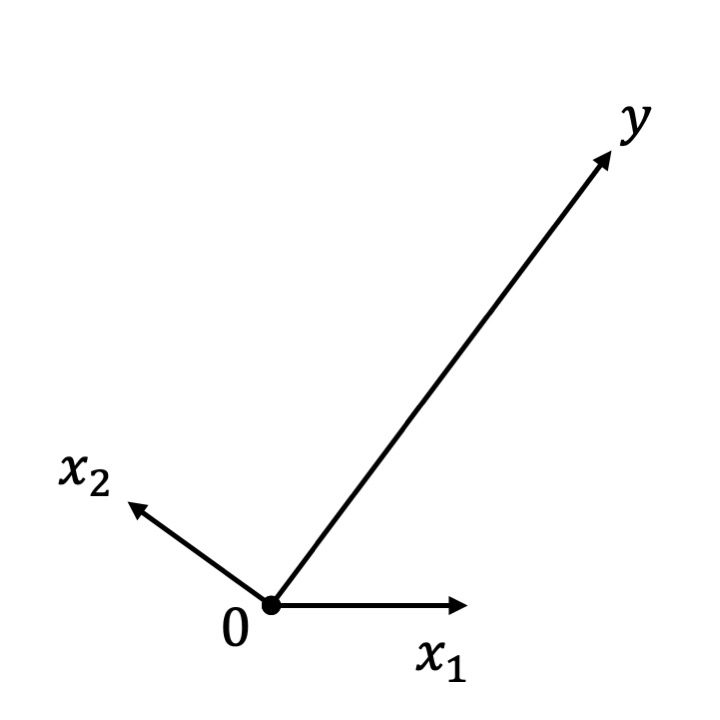
\includegraphics[width=0.95\textwidth]{img/FStepR/1.jpeg}
        \end{center}
    \end{figure}
\end{columns}
\end{frame}

\begin{frame}
\frametitle{Forward Stepwise Selection}
A simple example in the case of $p=2$ predictors.

\begin{columns}
    \column{0.5\textwidth}
    \begin{enumerate}
        \item Start with a null model.
        \item Find the predictor most correlated with the response and perform simple linear regression.
    \end{enumerate}
    
    \column{0.5\textwidth}
    \begin{figure}[!htbp]
        \begin{center}
            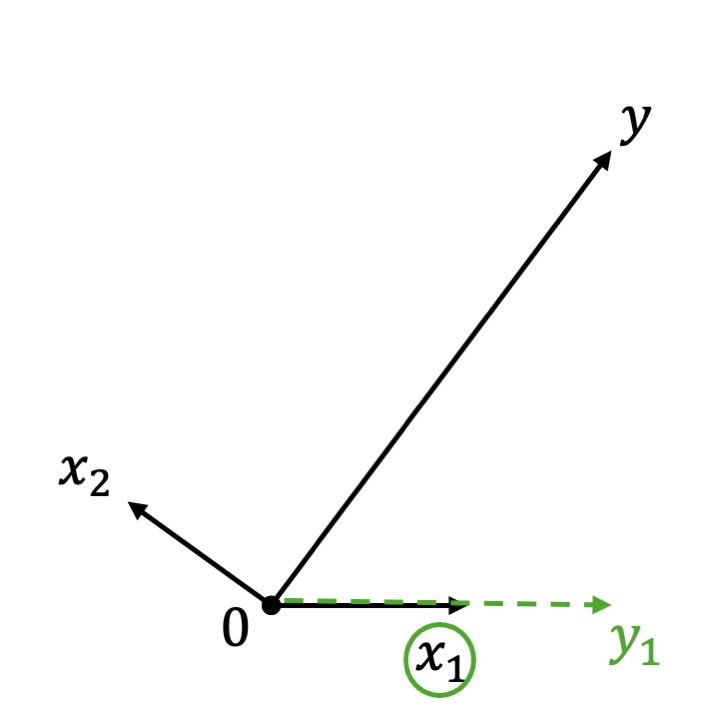
\includegraphics[width=0.95\textwidth]{img/FStepR/2.jpeg}
        \end{center}
        % \caption{Regression with Forward Stepwise Selection}
    \end{figure}
    \end{columns}
\end{frame}

\begin{frame}
\frametitle{Forward Stepwise Selection}
A simple example in the case of $p=2$ predictors.

\begin{columns}
    \column{0.5\textwidth}
    \begin{enumerate}
        \item Start with a null model.
        \item Find the predictor most correlated with the response and perform simple linear regression.
        \item Set the residuals as the new response.
    \end{enumerate}
    
    \column{0.5\textwidth}
    \begin{figure}[!htbp]
        \begin{center}
            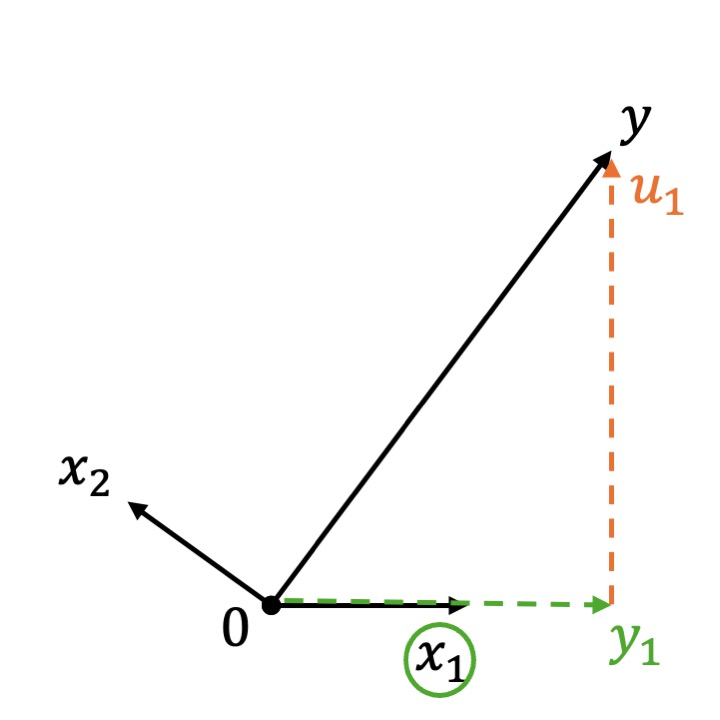
\includegraphics[width=0.95\textwidth]{img/FStepR/3.jpeg}
        \end{center}
        % \caption{Regression with Forward Stepwise Selection}
    \end{figure}
    \end{columns}
\end{frame}

\begin{frame}
\frametitle{Forward Stepwise Selection}
A simple example in the case of $p=2$ predictors.

\begin{columns}
    \column{0.5\textwidth}
    \begin{enumerate}
        \item Start with a null model.
        \item Find the predictor most correlated with the response and perform simple linear regression.
        \item Set the residuals as the new response.
        \item Project other predictors orthogonal to the predictor selected in previous step.
    \end{enumerate}
    
    \column{0.5\textwidth}
    \begin{figure}[!htbp]
        \begin{center}
            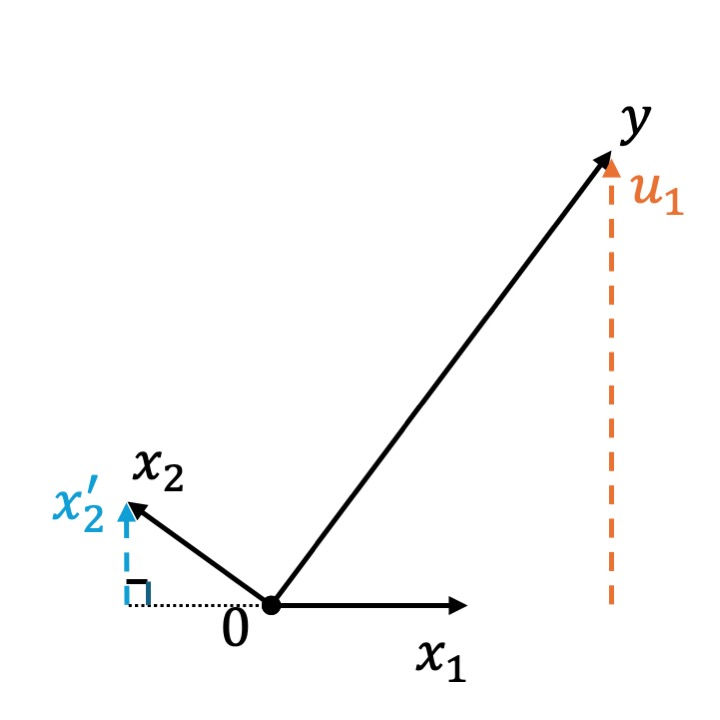
\includegraphics[width=0.95\textwidth]{img/FStepR/4.jpeg}
        \end{center}
        % \caption{Regression with Forward Stepwise Selection}
    \end{figure}
    \end{columns}
\end{frame}

\begin{frame}
\frametitle{Forward Stepwise Selection}
A simple example in the case of $p=2$ predictors.

\begin{columns}
    \column{0.5\textwidth}
    \begin{enumerate}
        \item Start with a null model.
        \item Find the predictor most correlated with the response and perform simple linear regression.
        \item Set the residuals as the new response.
        \item Project other predictors orthogonal to the predictor selected in previous step.
        \item Repeat steps $2-4$ until the stopping criterion is met.
    \end{enumerate}
    
    \column{0.5\textwidth}
    \begin{figure}[!htbp]
        \begin{center}
            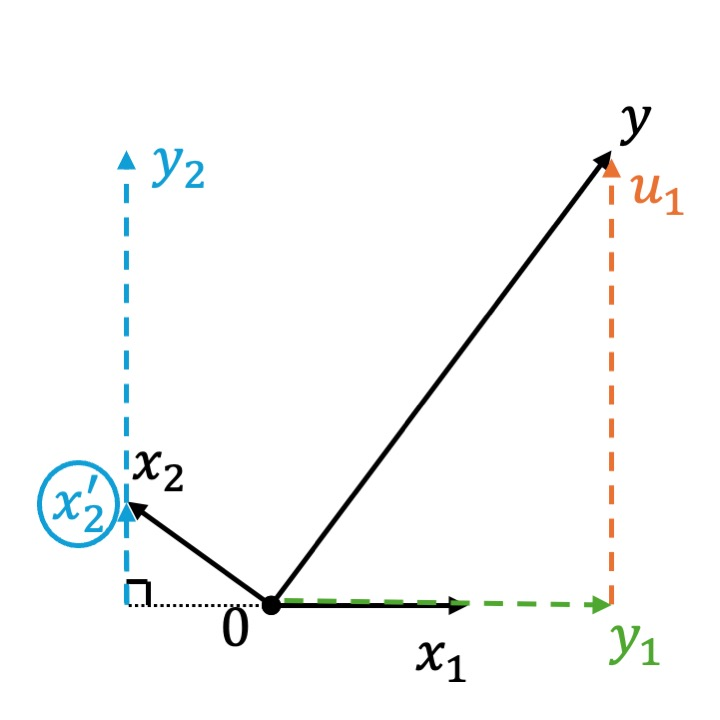
\includegraphics[width=0.95\textwidth]{img/FStepR/5.jpeg}
        \end{center}
        % \caption{Regression with Forward Stepwise Selection}
    \end{figure}
    \end{columns}
\end{frame}

%---------------------------------------------------------
\begin{frame}
\frametitle{Forward Stagewise Selection}
In contrast to forward stepwise selection, forward stagewise selection builds the model in successive small steps $\varepsilon$.

\begin{columns}
    \column{0.5\textwidth}
    Let $\hat{\mathbf{\mu}}$ be the current Stagewise estimate and $\hat{\mathbf{c}}=\mathbf{c}(\hat{\mathbf{\mu}})=X^T(y-\hat{\mathbf{\mu}})$ be the vector of current correlations. Therefore, $\hat{c}_j$ is proportional to the correlation between the covariate $x_j$ and the current residual vector.
    \begin{enumerate}
        \item Start with $\hat{\mathbf{\mu}}=0$.
    \end{enumerate}
    
    \column{0.5\textwidth}
    \begin{figure}[!htbp]
        \begin{center}
            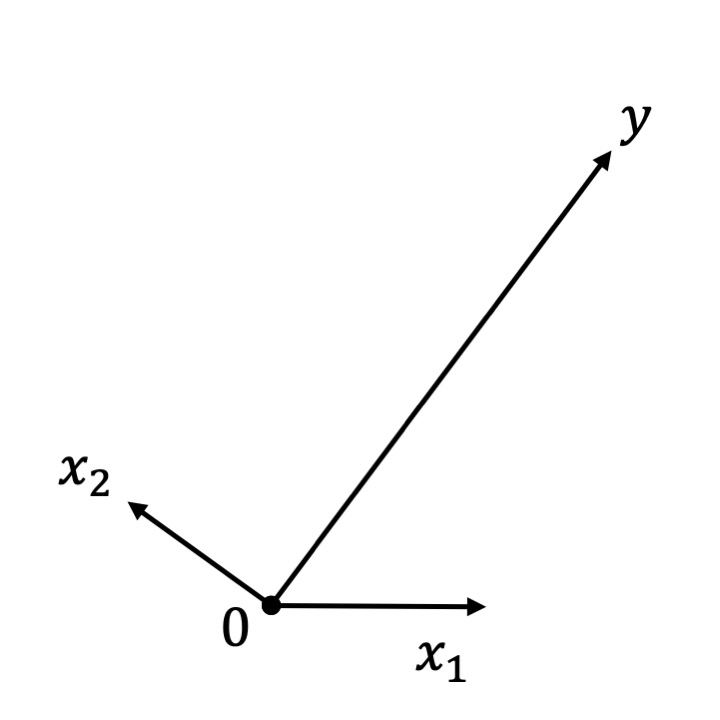
\includegraphics[width=0.95\textwidth]{img/FStageR/1.jpeg}
        \end{center}
    \end{figure}
\end{columns}
\end{frame}

\begin{frame}
\frametitle{Forward Stagewise Selection}
Let $\hat{\mathbf{\mu}}$ be the current Stagewise estimate and $\hat{\mathbf{c}}=\mathbf{c}(\hat{\mathbf{\mu}})=X^T(y-\hat{\mathbf{\mu}})$ be the vector of current correlations.

\begin{columns}
    \column{0.5\textwidth}
    \begin{enumerate}
        \item Start with $\hat{\mathbf{\mu}}=0$.
        \item Find the predictor $j$ that has the highest correlation that $\hat{j}=\arg\max_{j}|\hat{c}_j|$.
        \item Update $\hat{\mathbf{\mu}}\leftarrow\hat{\mathbf{\mu}}+\varepsilon\cdot\text{sign}(\hat{c}_{\hat{j}})\cdot\mathbf{x}_{\hat{j}}$ and $\mathbf{\hat{c}}$.
        \item Repeat steps $2-3$ until the stopping criterion is met.
    \end{enumerate}
    
    \column{0.5\textwidth}
    \begin{figure}[!htbp]
        \begin{center}
            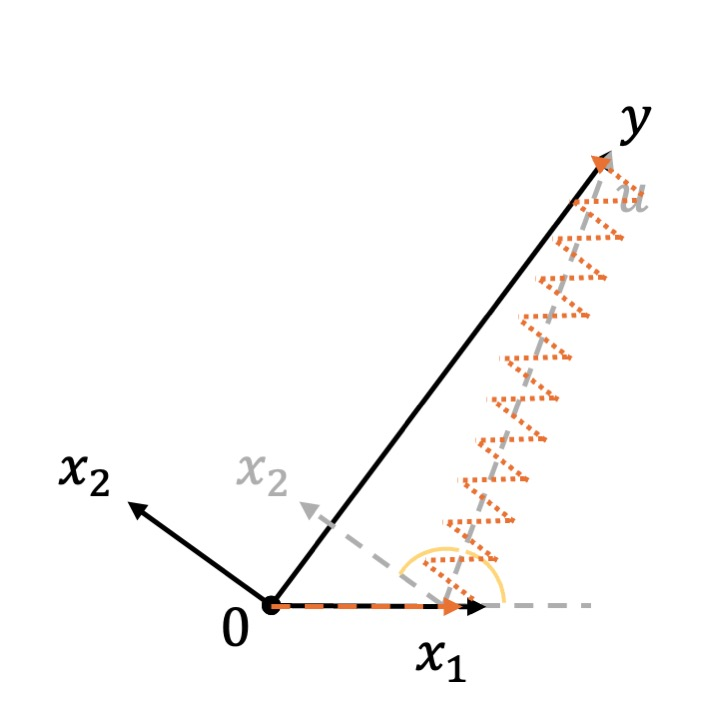
\includegraphics[width=0.95\textwidth]{img/FStageR/2.jpeg}
        \end{center}
    \end{figure}
\end{columns}
\end{frame}

%---------------------------------------------------------
\begin{frame}
\frametitle{Least Angle Regression}
Least Angle Regression (LARS) is a stylized version of forward stagewise procedure that uses a simple mathematical formula to accelerate the computations. Here shows the idea of LARS.

\begin{columns}
    \column{0.5\textwidth}
    \begin{enumerate}
        \item Start with all coefficients equal to zero.
    \end{enumerate}
    
    \column{0.5\textwidth}
    \begin{figure}[!htbp]
        \begin{center}
            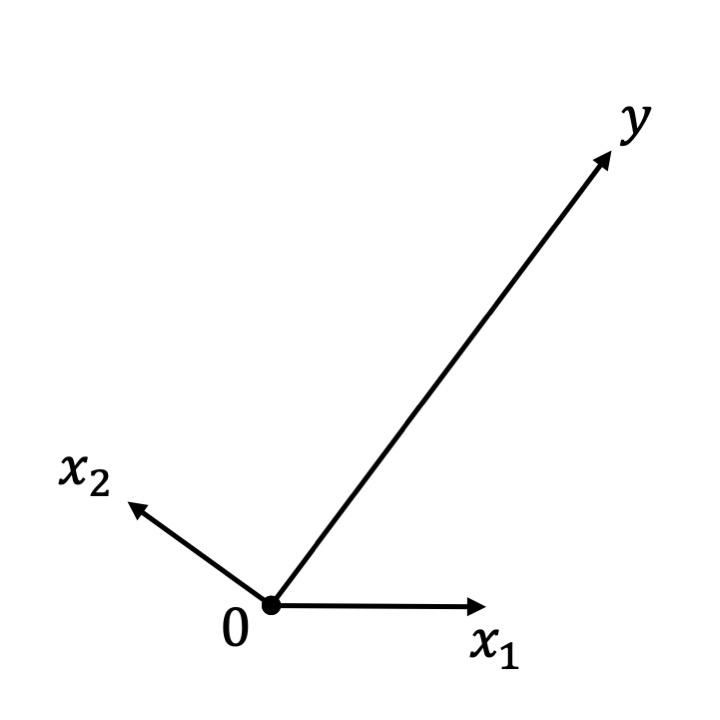
\includegraphics[width=0.95\textwidth]{img/LAR/1.jpeg}
        \end{center}
    \end{figure}
\end{columns}
\end{frame}

\begin{frame}
\frametitle{Least Angle Regression}
\begin{columns}
    \column{0.5\textwidth}
    \begin{enumerate}
        \item Start with all coefficients equal to zero.
        \item Find the predictor most correlated with the response.
    \end{enumerate}
    
    \column{0.5\textwidth}
    \begin{figure}[!htbp]
        \begin{center}
            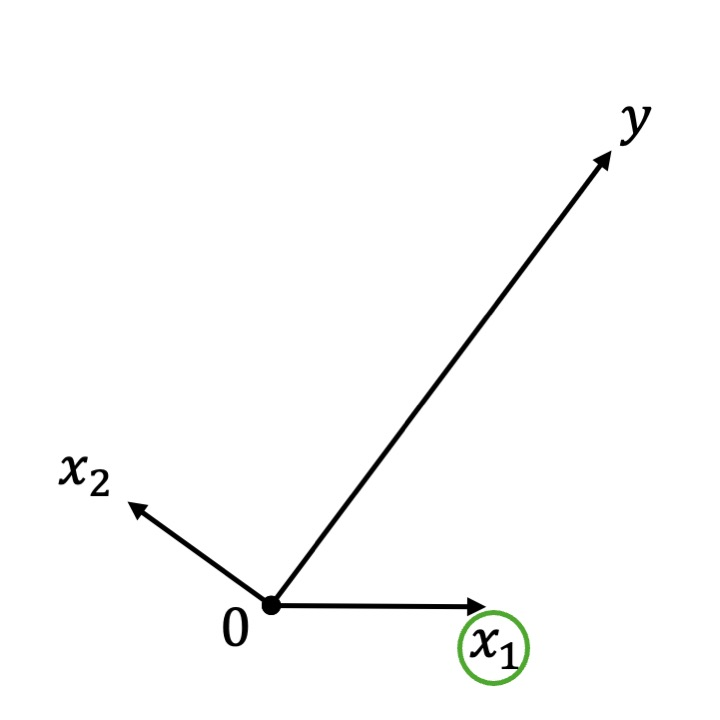
\includegraphics[width=0.95\textwidth]{img/LAR/2.jpeg}
        \end{center}
    \end{figure}
\end{columns}
\end{frame}

\begin{frame}
\frametitle{Least Angle Regression}
\begin{columns}
    \column{0.5\textwidth}
    \begin{enumerate}
        \item Start with all coefficients equal to zero.
        \item Find the predictor most correlated with the response.
        \item Take the largest step possible in the direction of this predictor until some other predictor has as much correlation with the current residual.
    \end{enumerate}
    
    \column{0.5\textwidth}
    \begin{figure}[!htbp]
        \begin{center}
            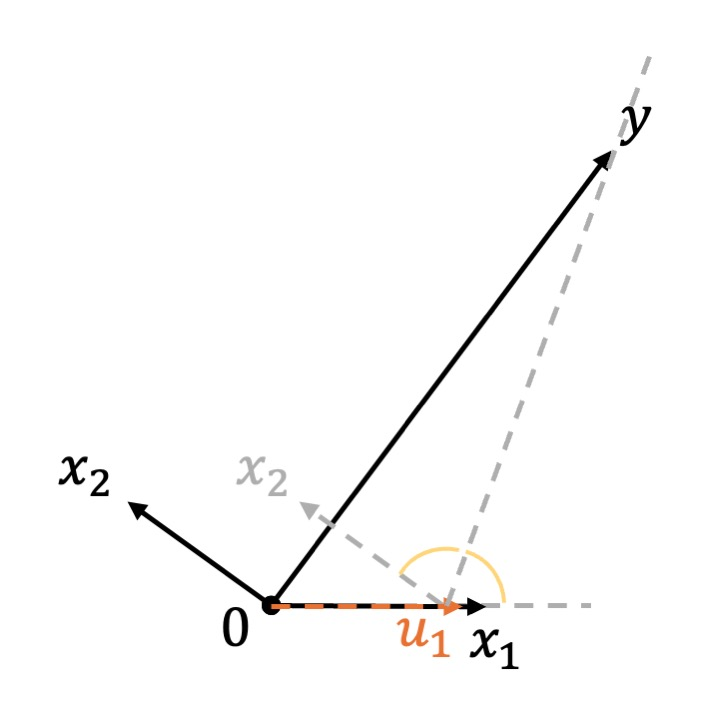
\includegraphics[width=0.95\textwidth]{img/LAR/3.jpeg}
        \end{center}
    \end{figure}
\end{columns}
\end{frame}

\begin{frame}
\frametitle{Least Angle Regression}
\begin{columns}
    \column{0.6\textwidth}
    \begin{enumerate}
        \item Start with all coefficients equal to zero.
        \item Find the predictor most correlated with the response.
        \item Take the largest step possible in the direction of this predictor until some other predictor has as much correlation with the current residual.
        \item The new direction is the equiangular vector of the two predictors. Move in until a third predictor earns its way into the ``most correlated'' set.
        \item Repeat steps $3-4$ until met the stopping criterion.
    \end{enumerate}
    
    \column{0.4\textwidth}
    \begin{figure}[!htbp]
        \begin{center}
            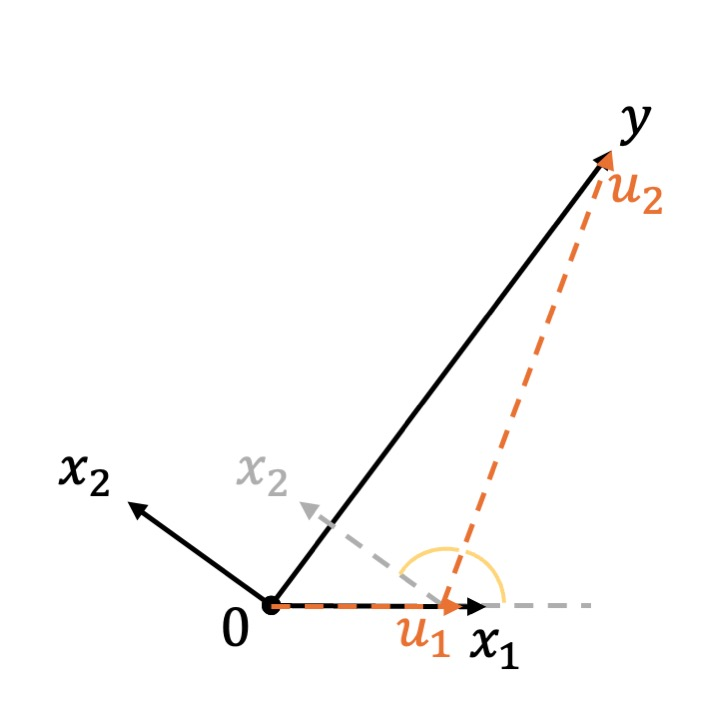
\includegraphics[width=0.95\textwidth]{img/LAR/4.jpeg}
        \end{center}
    \end{figure}
\end{columns}
\end{frame}

\begin{frame}
\frametitle{Least Angle Regression}
Assume that $\mathbf{x}_1,\dots,\mathbf{x}_p$ are linearly independent and for $\mathcal{A}$ a subset of indices $\{1,\dots,p\}$, define the matrix $\mathbf{X}_\mathcal{A}={(\dots,s_j\mathbf{x}_j,\dots)}_{j\in\mathcal{A}}$ where signs $s_j$ equal $\pm 1$. Let
\begin{equation}
    \g_\mathcal{A}=\mathbf{X}_\mathcal{A}^T\mathbf{X}_\mathcal{A}
    \quad \text{and} \quad
    A_\mathcal{A}={(\mathbf{1}^T_\mathcal{A}\g^{-1}_\mathcal{A}\mathbf{1}_\mathcal{A})}^{-1/2},\label{eq:lars25}
\end{equation}
where $\mathbf{1}_\mathcal{A}$ is a vector of ones of length $|\mathcal{A}|$. The equiangular vector $\mathbf{u}_\mathcal{A}$ is defined as
\begin{equation}
    \mathbf{u}_\mathcal{A}=\mathbf{X}_\mathcal{A} A_\mathcal{A}\g^{-1}_\mathcal{A}\mathbf{1}_\mathcal{A},\label{eq:lars26}
\end{equation}
is the unit vector making equal angles, less than $90^\circ$, with the columns of $\mathbf{X}_\mathcal{A}$ satisfying $\mathbf{X}_\mathcal{A}^T\mathbf{u}_\mathcal{A}=A_\mathcal{A}\mathbf{1}_\mathcal{A}$ and $\|\mathbf{u}_\mathcal{A}\|=1$.
\end{frame}

\begin{frame}
\frametitle{Least Angle Regression}
Then the algorithm of LARS comes as follows:
\begin{enumerate}
    \item Initialize all the coefficients as 0, the residual $\mathbf{u}=\mathbf{y}$ and the active set $\mathcal{A}=\emptyset$.
    \item Suppose that $\hat{\mathbf{\mu}}_\mathcal{A}$ is the current estimate of the response and $\hat{\mathbf{c}}=\mathbf{c}(\hat{\mathbf{\mu}}_\mathcal{A})=X^T(y-\hat{\mathbf{\mu}}_\mathcal{A})$ are the current correlations. The active set $\mathcal{A}$ is the set of indices corresponding to covariates with the greatest absolute correlations, i.e., $\mathcal{A}=\{j:|\hat{c}_j|=\hat{\mathbf{C}}\}$ and $\hat{\mathbf{C}}=\max_{j}|\hat{c}_j|$.
    
    Let $s_j=\text{sign}(\hat{c}_j)$ for $j\in\mathcal{A}$, and compute $A_\mathcal{A}$, and $\mathbf{u}_\mathcal{A}$ as in \ref{eq:lars25} and \ref{eq:lars26}. Also, compute the inner product $\mathbf{a}=:X^T\mathbf{u}_\mathcal{A}$. Updates $\hat{\mathbf{\mu}}_\mathcal{A}$ as 
    $$\hat{\mathbf{\mu}}_\mathcal{A}\leftarrow\hat{\mathbf{\mu}}_\mathcal{A}+\hat{\gamma}\mathbf{u}_\mathcal{A},$$
    where $\hat{\gamma}=\min_{j\in\mathcal{A}^c}^+\left(\frac{\hat{\mathbf{C}}-\hat{c}_j}{A_\mathcal{A}-\mathbf{a}_j}, \frac{\hat{\mathbf{C}}+\hat{c}_j}{A_\mathcal{A}+\mathbf{a}_j}\right)$; ``$\min^+$'' denotes the minimum taken over only positive quantities.
    \item Repeat step 2 until the stopping criterion is met.
\end{enumerate}
    
\end{frame}

\begin{frame}
    \frametitle{Comparison of LARS and Forward Stagewise Selection}
\begin{figure}[!htbp]
    \begin{center}
        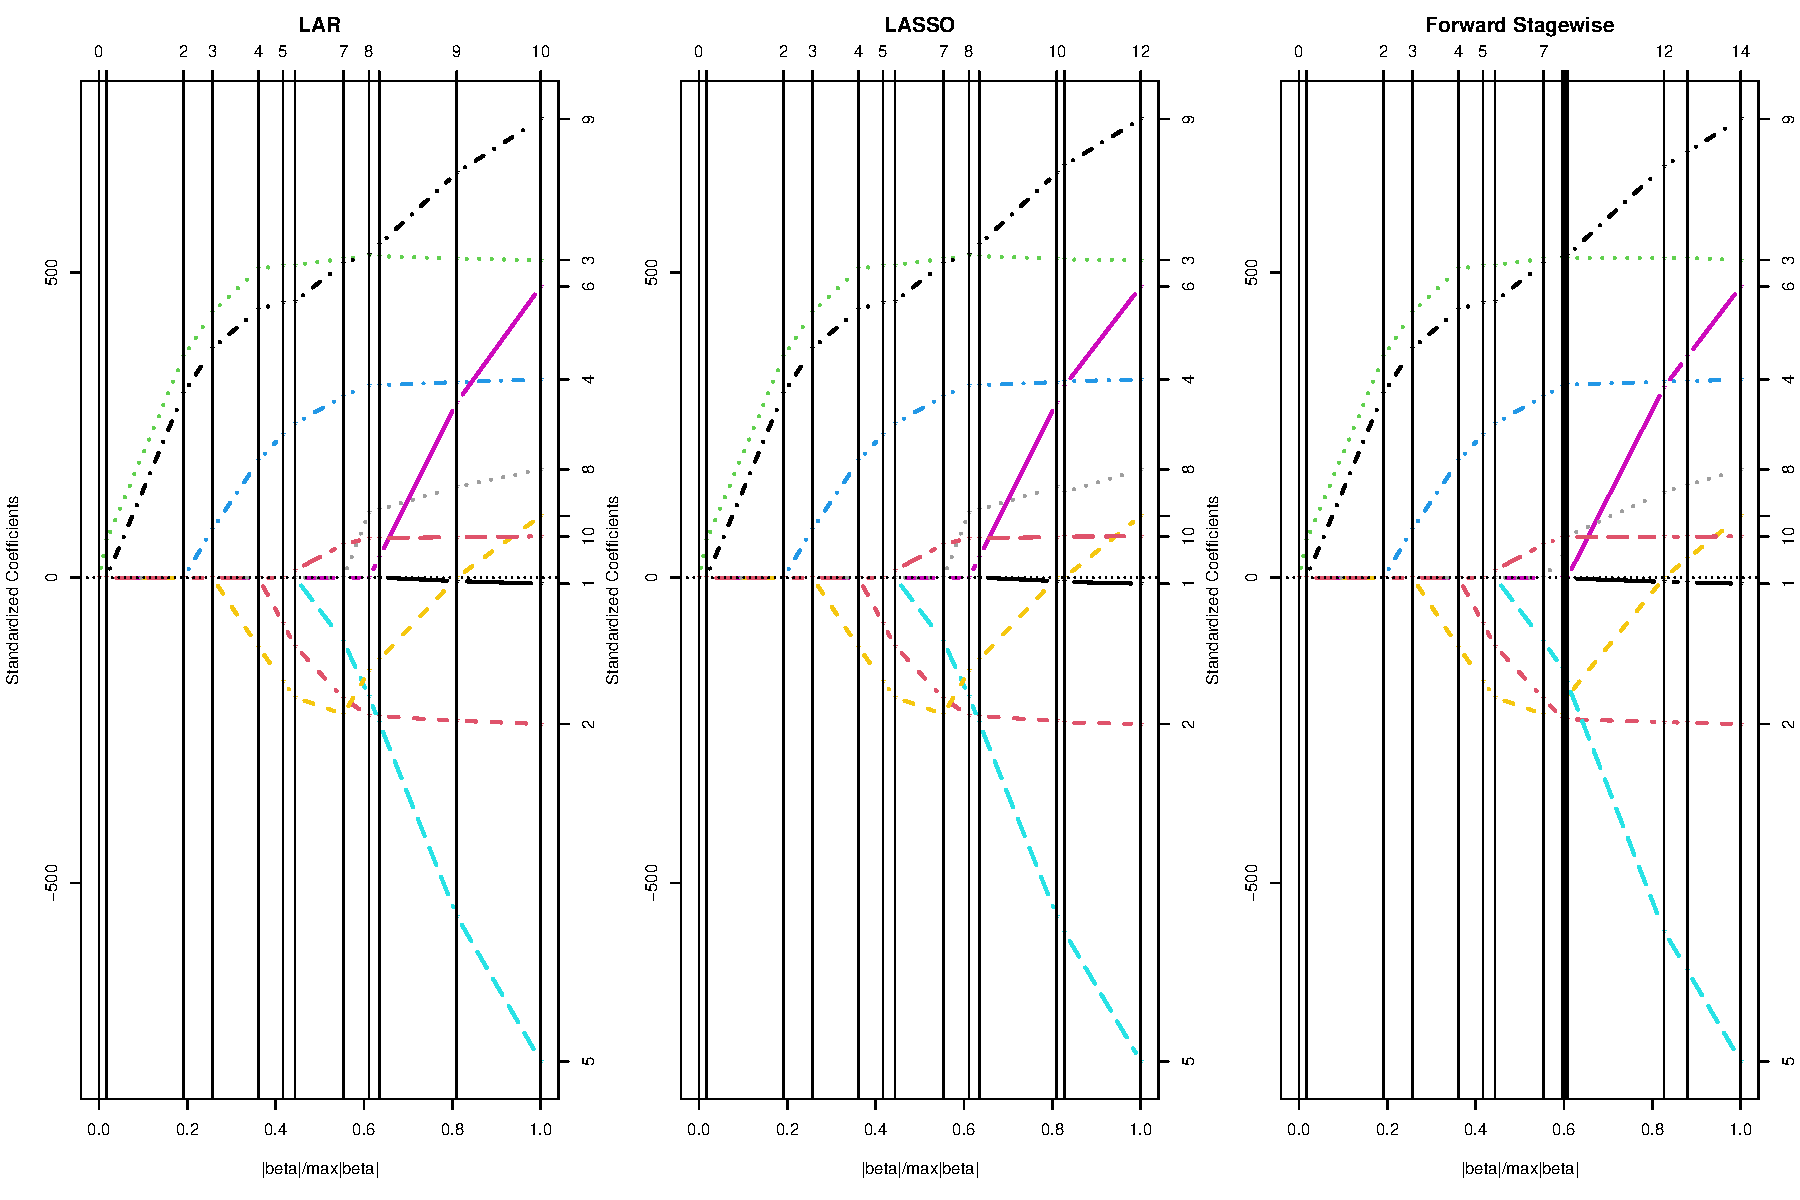
\includegraphics[width=0.95\textwidth]{img/lars_diabetes.pdf}
    \end{center}
    \caption{Estimation paths of LARS and Forward Stagewise Selection for the diabetes data set.}
    \label{fig:lars_diabetes}
\end{figure}
\end{frame}

\section{Coordinate Descent}
% In this slide, some important text will be
% \alert{highlighted} because it's important.
% Please, don't abuse it.

% \begin{block}{Remark}
% Sample text
% \end{block}

% \begin{alertblock}{Important theorem}
% Sample text in red box
% \end{alertblock}

% \begin{examples}
% Sample text in green box. The title of the block is ``Examples".
% \end{examples}